\apendice{Documentación de usuario}

\section{Introducción}
En este anexo se describen los requisitos \emph{hardware} y \emph{software} que debe cumplir cualquier usuario que desee hacer uso de la aplicación, así como un manual de uso de la aplicación. Además, se ha realizado un vídeo-tutorial que se puede consultar completo en:

\url{https://www.youtube.com/playlist?list=PLM0y-okbdAOGkw9JrtwosMJ5bfMa3aNX8}

\section{Requisitos de usuarios}
El objetivo final de la aplicación es que sea una aplicación Web, desplegada en un servidor accesible vía Internet. El usuario solo deberá disponerse un equipo con un navegador actualizado y conexión a Internet.
Se ha testeado el funcionamiento de la aplicación en los siguientes navegadores:
\begin{itemize}
\item \emph{Google Chrome} Versión 74.0.3729.169 (Build oficial) (64 bits)
\item Microsoft Edge 42.17134.1.0
\item Firefox Quantum 67.0 (64-bits)

\end{itemize}

Otra opción es si el usuario desea tenerlo instalado en su equipo, en este caso solo necesita disponer de las herramientas \emph{Docker} y \emph{Docker Compose} instaladas. Hay que mencionar que \emph{Docker} no funciona en la versión de \emph{Windows 10 Home Edition}, no es compatible con la tecnología de virtualización  \emph{Hyper-V}. Existe la posibilidad de usar la herramienta \emph{Docker Toolbox}\footnote{\textsl{Docker Toolbox}: \url{https://docs.docker.com/toolbox/toolbox_install_windows/}}, pero no se garantiza su correcto funcionamiento en todos los casos. \emph{Docker} funciona perfectamente con las versiones \emph{Windows 10 Pro} y \emph{Windows 10 Enterprise}.

En \emph{Linux} y \emph{Mac}, su funcionamiento es correcto.

\section{Instalación}
Si se desea instalar en un equipo, hay que seguir las instrucciones detalladas en el apartado, \ref{sec:instalacion}~\textbf{Compilación, instalación y ejecución del proyecto}, en la página~\pageref{sec:instalacion}. También se pueden consultar en el archivo  \texttt{README.md} del repositorio de \emph{GitHub}.

\section{Manual del usuario}

En esta sección se describe el uso de las diferentes funcionalidades de la aplicación.
\subsection{Acceso a la aplicación.}
Cuando se accede a la aplicación se nos informa del uso de las \emph{cookies} mediante un mensaje. 

\begin{figure}[H]
	\centering
	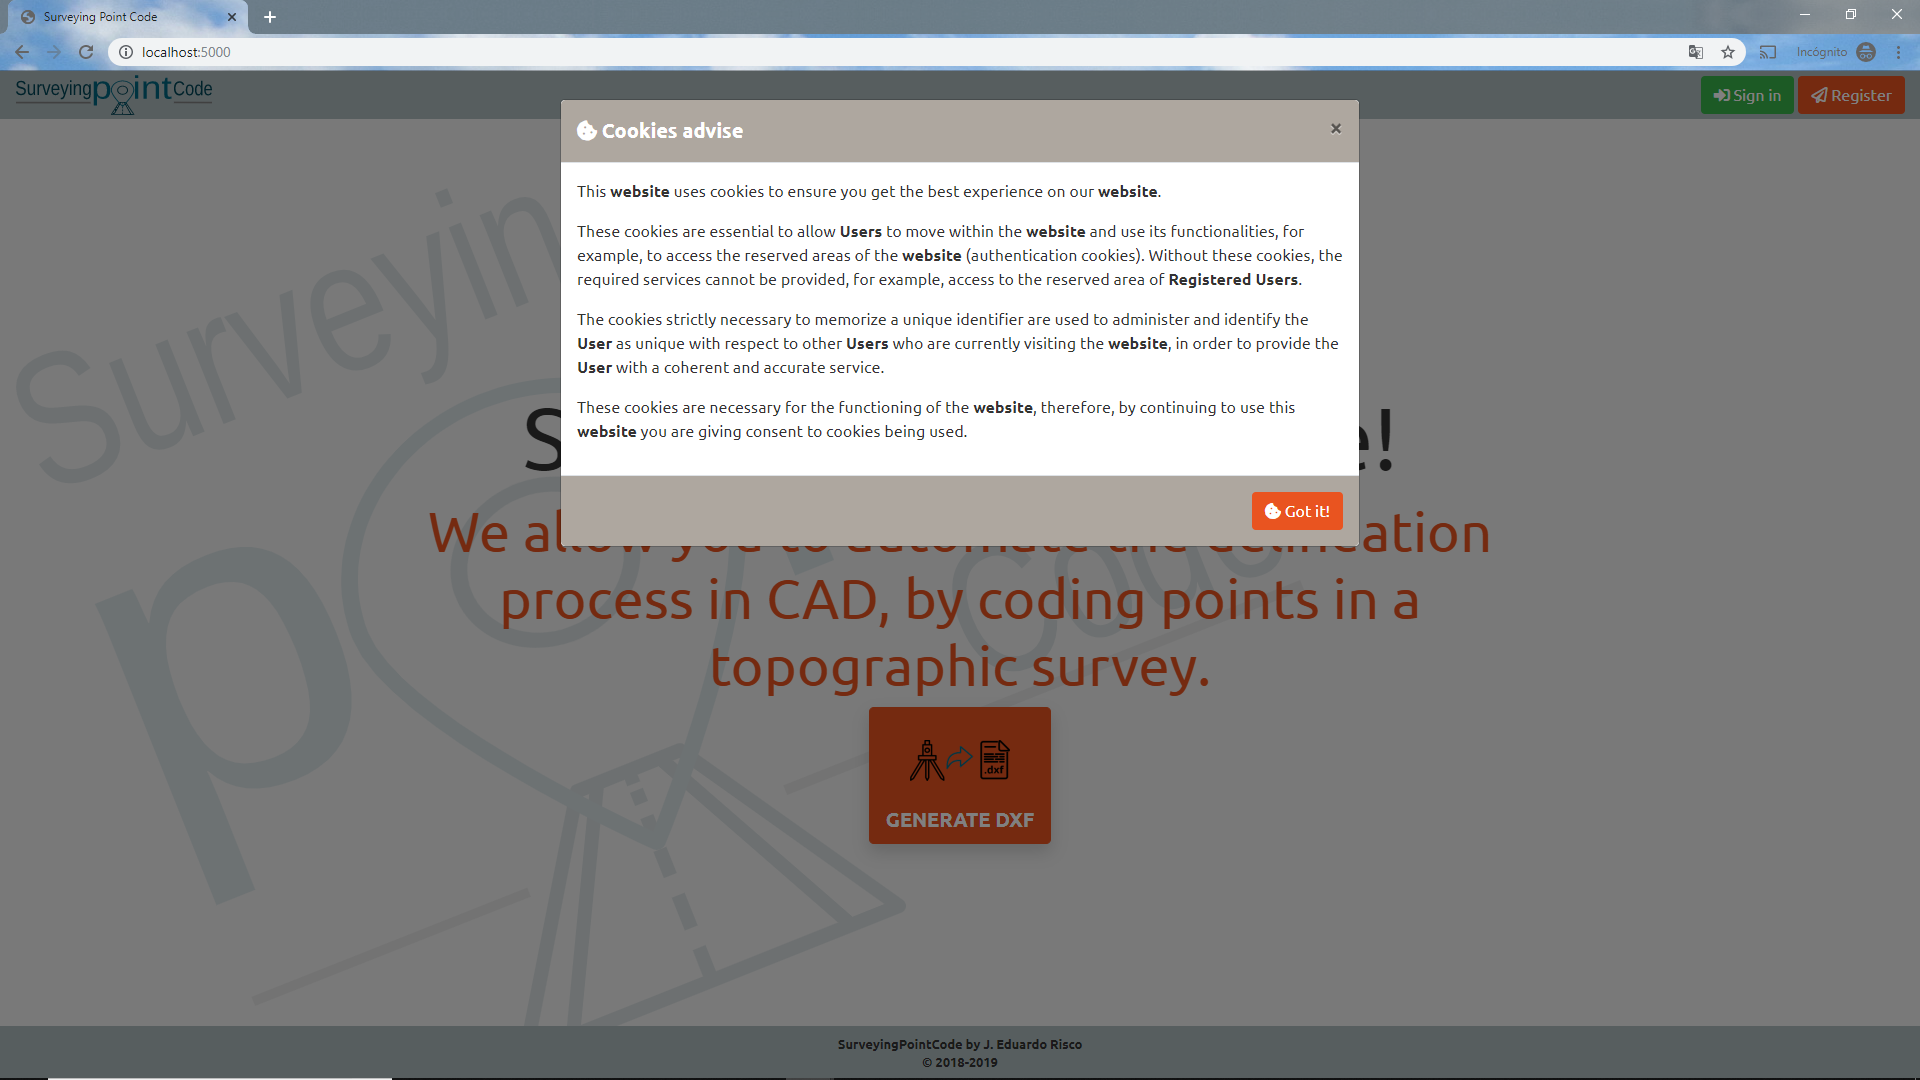
\includegraphics[width=1\textwidth]{M_01}
	\caption{Mensaje de información \emph{cookies}.}
	\label{fig:M_01}
\end{figure}

Cerramos el mensaje y tenemos pantalla de bienvenida de la aplicación. En ella tenemos varias posibilidades:

\begin{itemize}
\item Si no estamos \emph{logeados}, podemos acceder a la pantalla de  \emph{login} pulsando el botón \textbf{Sign in}.
\item Si no estamos \emph{logeados}, podemos acceder a la pantalla de  registro pulsando el botón \textbf{Register}.
\item Si pulsamos el botón \textbf{GENERATE DXF} y no estamos \emph{logeados}, accedemos a la pantalla de \emph{login} y si estamos   \emph{logeados} accedemos a la pantalla de \emph{Upload files}.

\end{itemize}

\begin{figure}
	\centering
	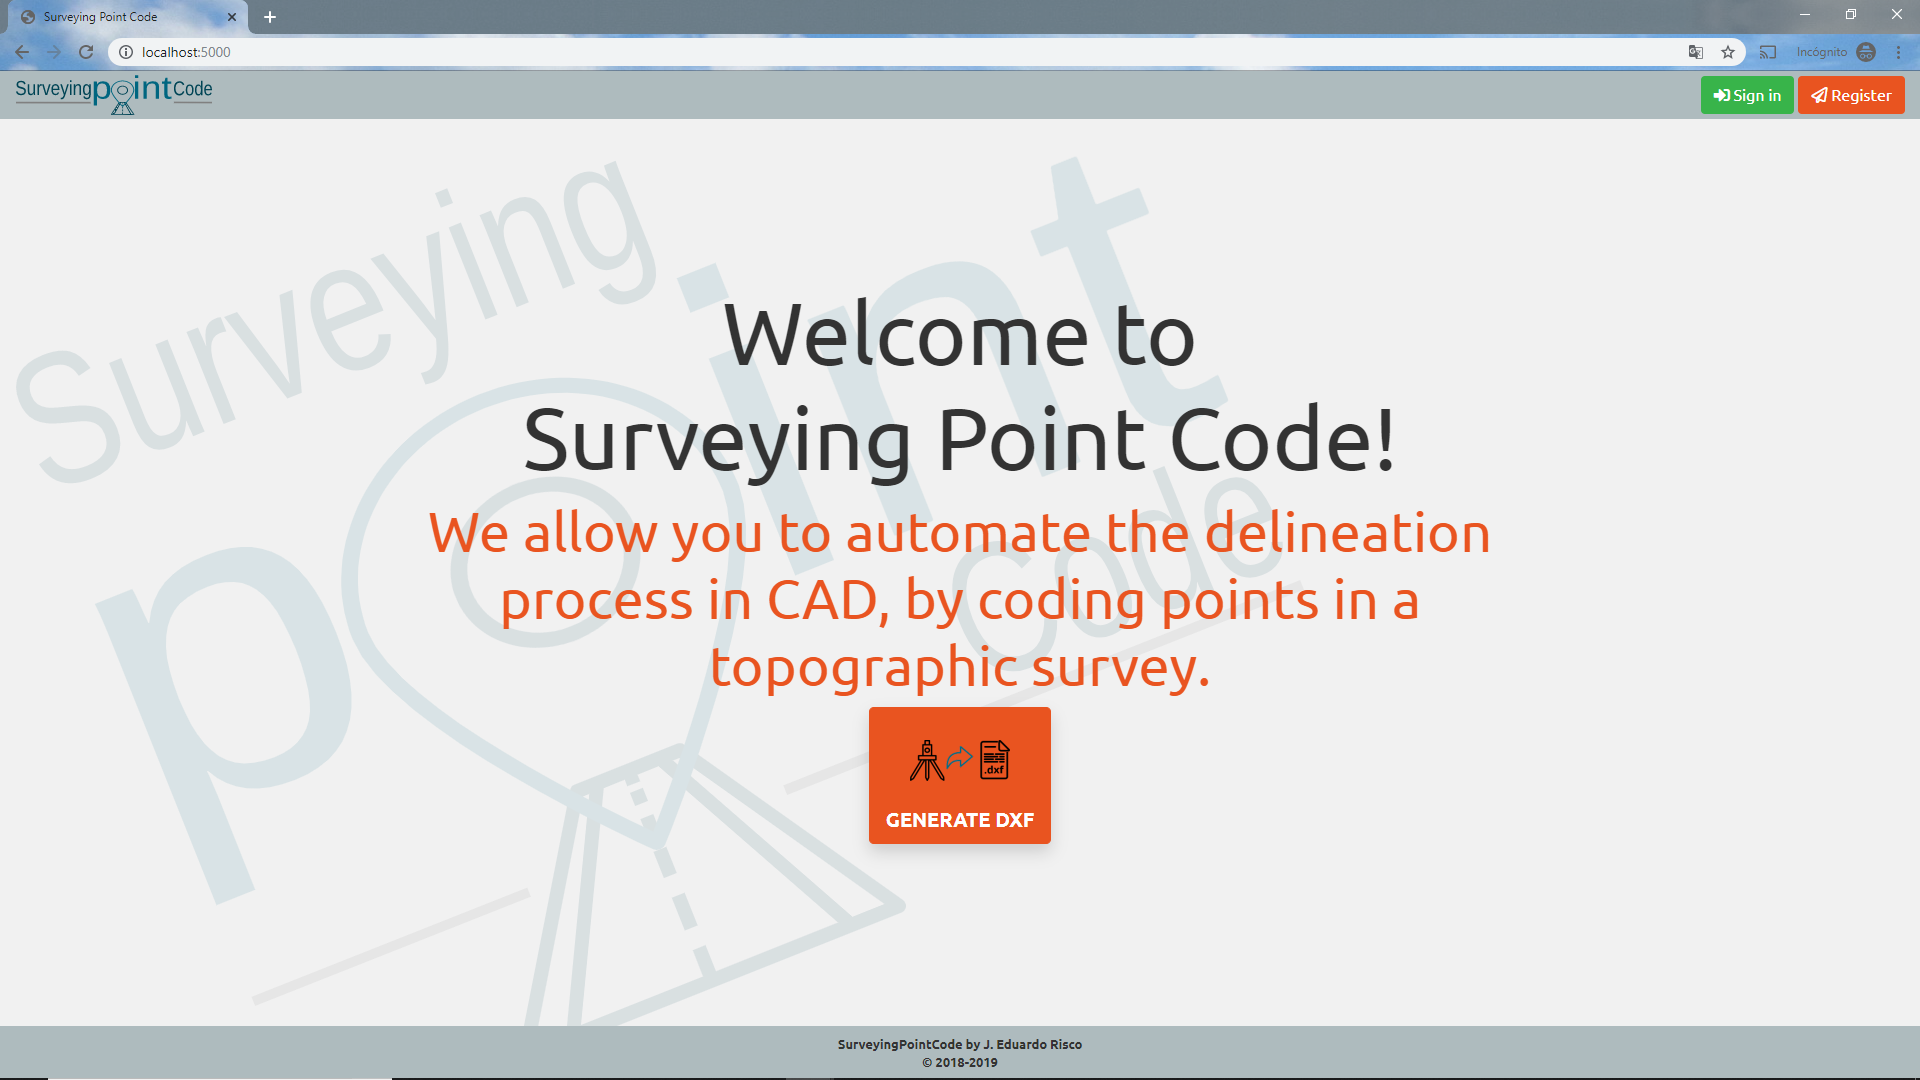
\includegraphics[width=1\textwidth]{M_02}
	\caption{Pantalla de bienvenida.}
	\label{fig:M_02}
\end{figure}

\newpage

\subsection{Registro de usuario.}



\begin{figure}[H]
	\centering
	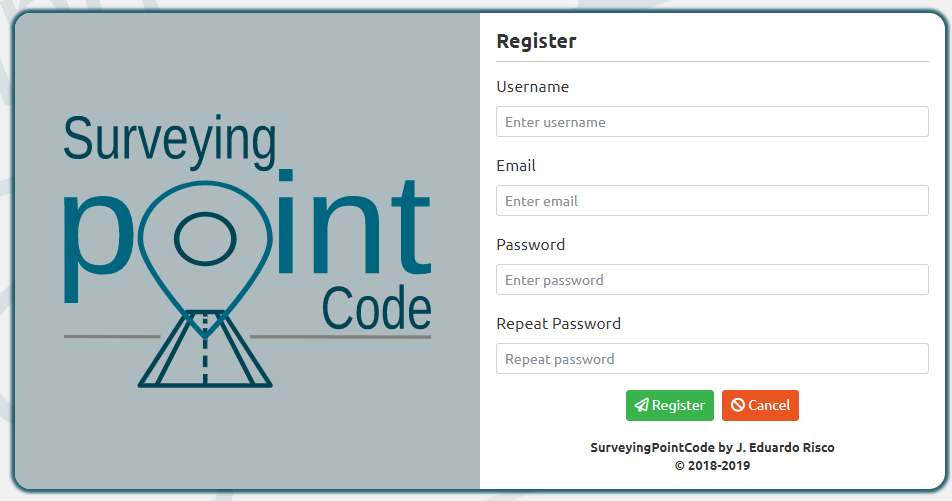
\includegraphics[width=0.6\textwidth]{M_04}
	\caption{Registro de usuario.}
	\label{fig:M_04}
\end{figure}

\textbf{\underline{Pasos para registrarse:} }

\begin{enumerate}

\item Introducir nombre de usuario.
\item Introducir e-mail.
\item Introducir contraseña.
\item Repetir contraseña.
\item Pulsar el botón \textbf{Register}.

Una vez completado el registro, la aplicación irá a la pantalla de \emph{login}, mostrando un mensaje informando que el registro se ha realizado con éxito.

\begin{figure}[H]
	\centering
	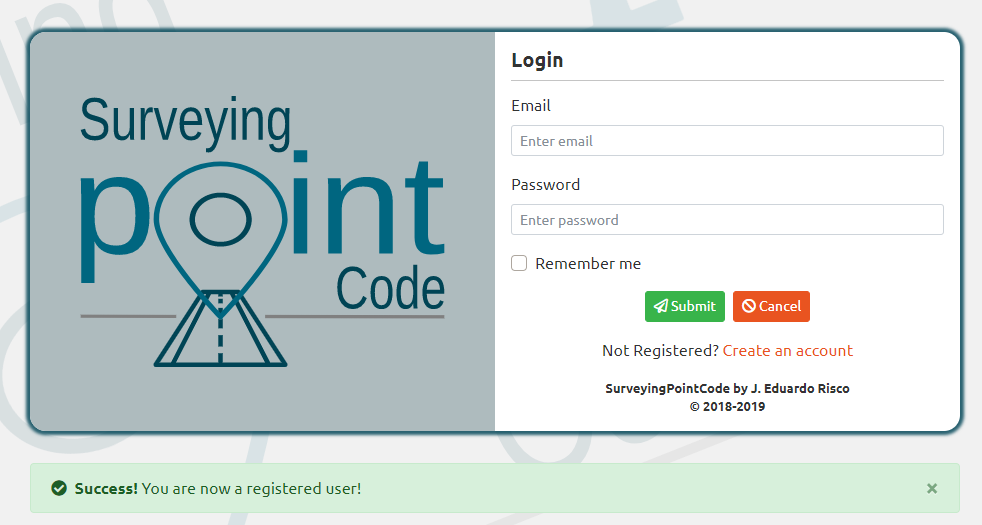
\includegraphics[width=0.6\textwidth]{M_04_M}
	\caption{Registro con éxito.}
	\label{fig:M_04_M}
\end{figure}

\end{enumerate}
\newpage

\textbf{\underline{Errores en el registro:} }



No se completará el registro y mostrará mensajes de error en los siguientes casos:

\begin{itemize}
\item El nombre de usuario ya existe.
\item El e-mail ya existe.
\item El e-mail no tiene un formato correcto de e-mail.
\item No coinciden las dos contraseñas introducidas.
\item No se hayan completado todos los campos requeridos.

\end{itemize}

\textbf{\underline{Otras opciones:} }
\begin{itemize}
\item Para salir de esta pantalla sin registrarse, pulsar el botón \textbf{Cancel}.
\end{itemize}

\subsection{\emph{Login} de usuario.}



\textbf{\underline{Pasos para \emph{logearse}:} }


\begin{figure}[H]
	\centering
	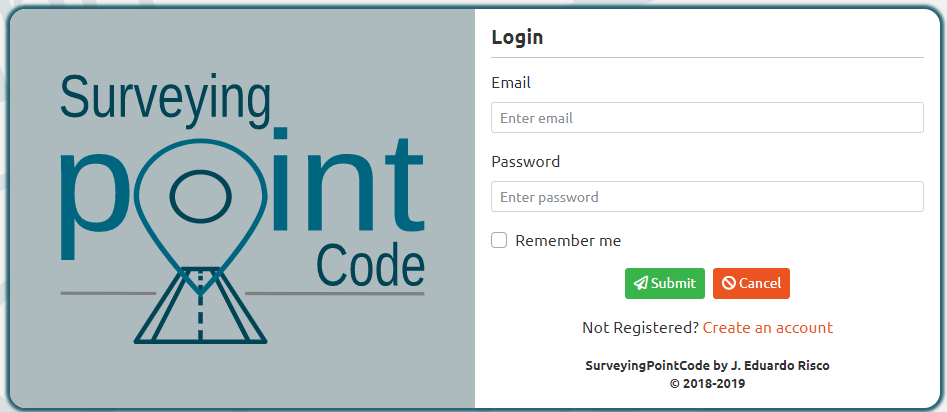
\includegraphics[width=0.7\textwidth]{M_03}
	\caption{\emph{Login} de usuario.}
	\label{fig:M_03}
\end{figure}


\begin{enumerate}

\item Introducir e-mail.
\item Introducir contraseña.
\item Pulsar el botón \textbf{Submit}.

Una vez \emph{logeado}, la aplicación irá a la pantalla de \emph{Upload files}.

\end{enumerate}
\newpage

\textbf{\underline{Errores en el \emph{login}:} }

No se completará el \emph{login} y mostrará mensajes de error en los siguientes casos:

\begin{itemize}
\item El nombre de usuario sea incorrecto.
\item El e-mail sea incorrecto.
\item No se hayan completado todos los campos requeridos.
\end{itemize}

\textbf{\underline{Otras opciones:} }

\begin{itemize}

\item Para salir de esta pantalla sin \emph{logearse}, pulsar el botón \textbf{Cancel}.
\item Para ir a la pantalla de registro, pulsar en el \emph{link} \textbf{Create an account}.

\end{itemize}


\subsection{Carga de archivos.}

El usuario tiene la opción de cargar 3 tipos de archivos: archivo topográfico, archivo de configuración de la conversión y archivo con símbolos. En los 3 casos el usuario puede buscar el archivo mediante el explorador que se abre al pulsar o arrastrar el archivo hasta la caja.

\begin{figure}[H]
	\centering
	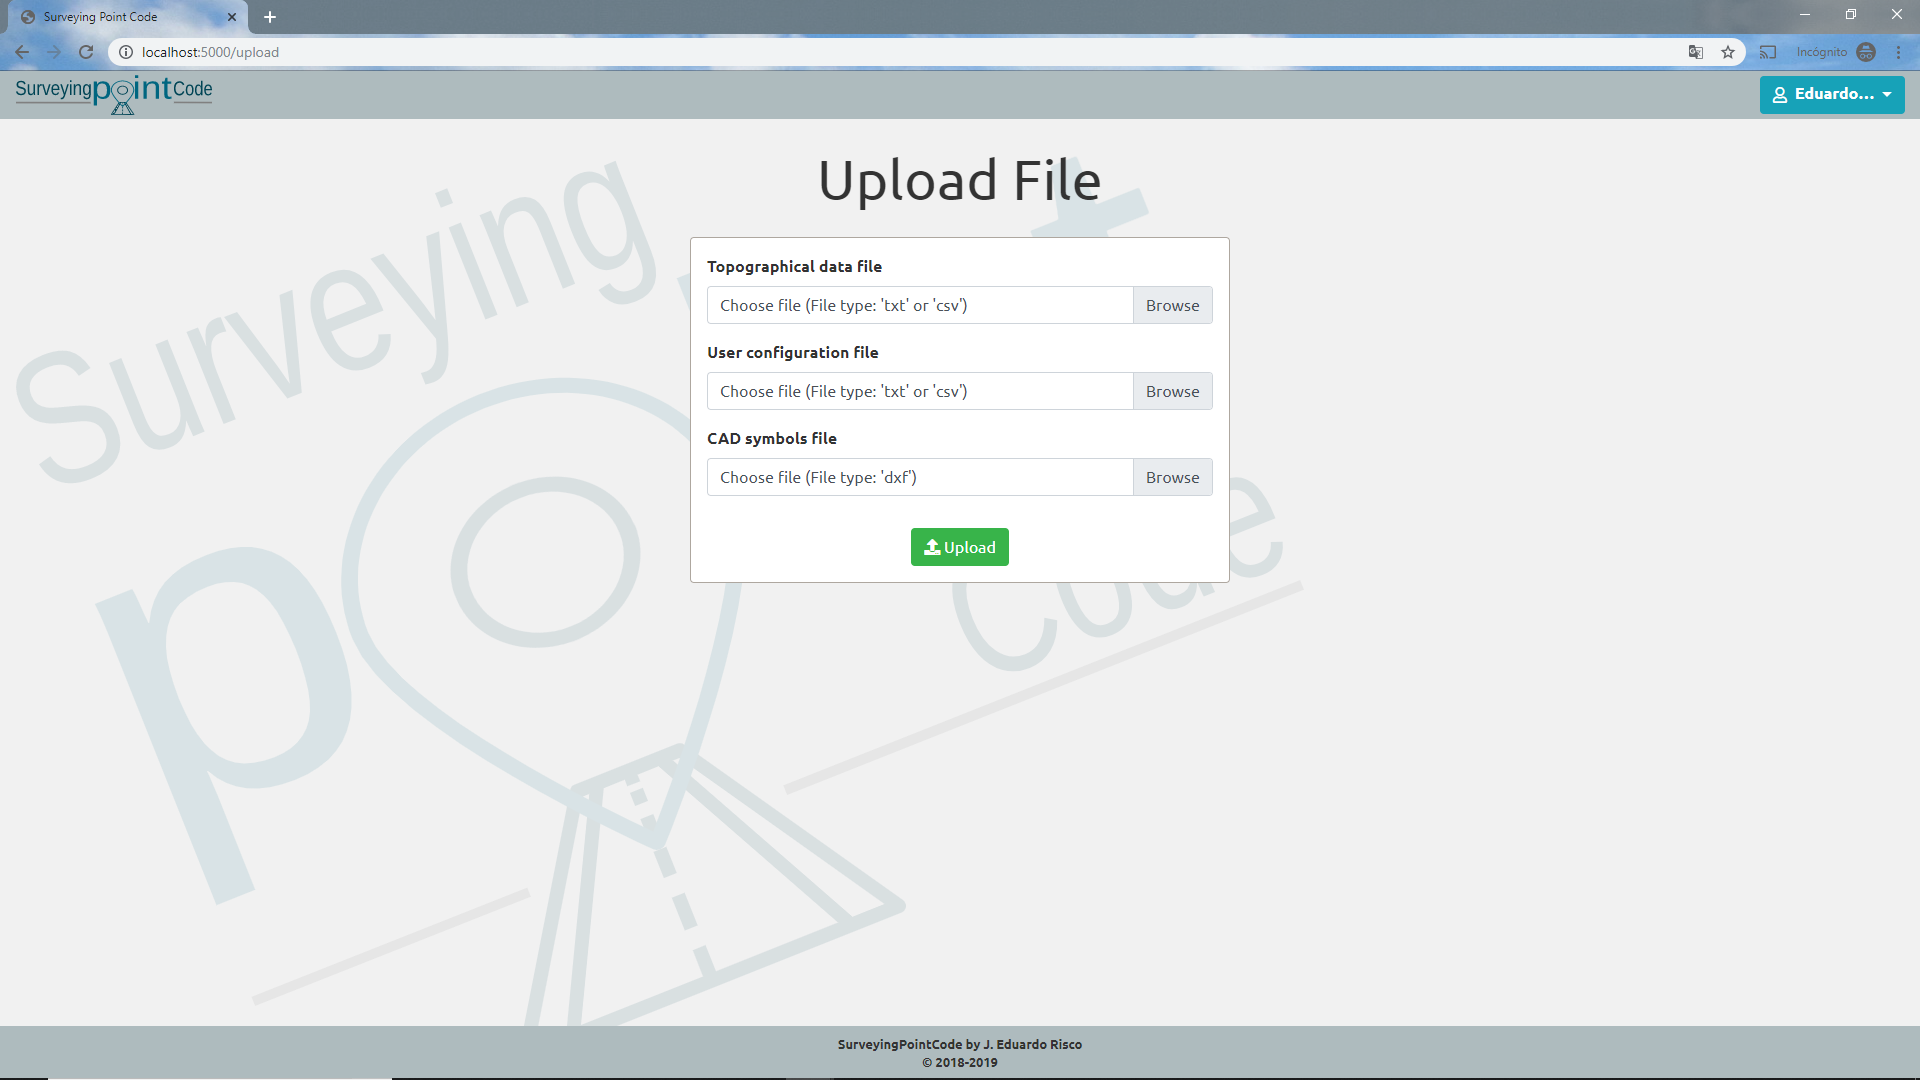
\includegraphics[width=1\textwidth]{M_05}
	\caption{Carga de archivos.}
	\label{fig:M_05}
\end{figure}

\subsubsection{Carga de archivo topográfico.}

El archivo topográfico es \textbf{obligatorio}. El archivo estará compuesto por una o varias líneas, cada línea equivale a un punto medido en campo. El punto obligatoriamente estará formado por los siguientes campos, separados por comas:
\begin{itemize}
\item Número de punto.
\item Coordenada $X$.
\item Coordenada $Y$.
\item Coordenada $Z$.
\item Código del punto.
\end{itemize}
La interpretación de la codificación se explica con detalle en el apartado <<3.3. Codificación de los puntos>>, de la memoria.



A continuación vemos un ejemplo de un archivo:

\begin{verbatim}
1,355776.180,4611015.011,691.055,E I
2,355773.203,4611028.546,691.055,E
3,355781.359,4611129.076,691.055,TR REG
4,355786.052,4611135.542,691.055,TC TEL
5,355783.215,4611143.179,691.055,TX 2 SAN
6,355754.037,4611145.893,691.055,A IC
7,355755.345,4611150.953,691.055,A C
8,355857.822,4611095.993,691.055,E -14.1 20.5 -25.75
\end{verbatim}

\textbf{\underline{Pasos para cargar un archivo topográfico:} }

\begin{enumerate}

\item Elegir un archivo topográfico.
\item Pulsar el botón \emph{Upload}

Si el archivo es correcto, la aplicación irá a la pantalla \emph{Convert File to DXF}.

\end{enumerate}

\textbf{\underline{Errores en la carga del archivo:} }

La carga no será correcta si al pulsar el botón \emph{Upload}, se presentan los siguientes errores:
\begin{itemize}



\item El archivo no tiene el formato correcto. En el mensaje aparecen las líneas del archivo donde están los errores. Se da la opción de volver a cargar el archivo, pulsando el botón \emph{Reload Files}.

\begin{figure}[H]
	\centering
	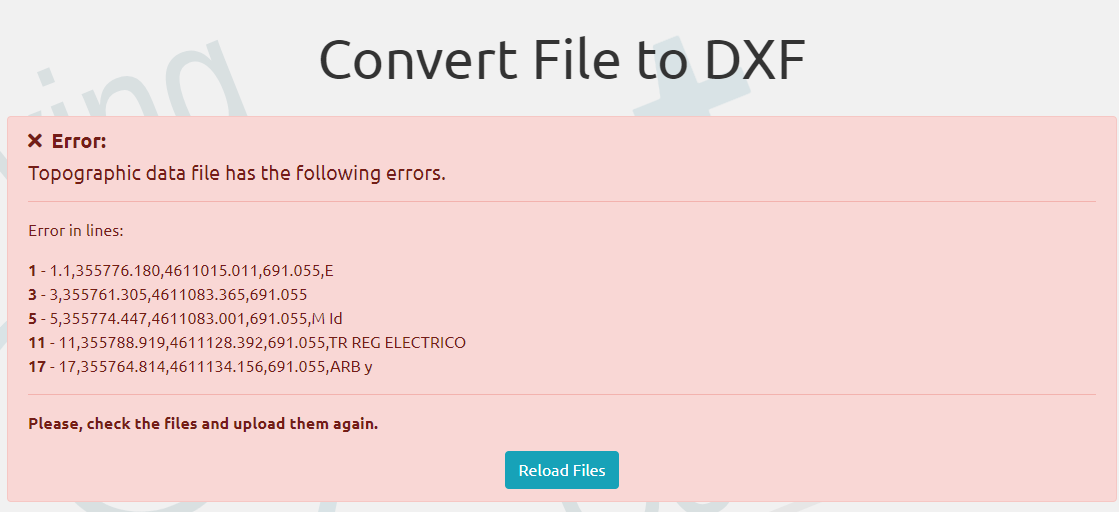
\includegraphics[width=0.7\textwidth]{M_07_E}
	\caption{Error formato de archivo topográfico, \emph{parser}.}
	\label{fig:M_07_E}
\end{figure}

\item El archivo está vacío. Se da la opción de volver a cargar el archivo, pulsando el botón \emph{Reload Files}.

\begin{figure}[H]
	\centering
	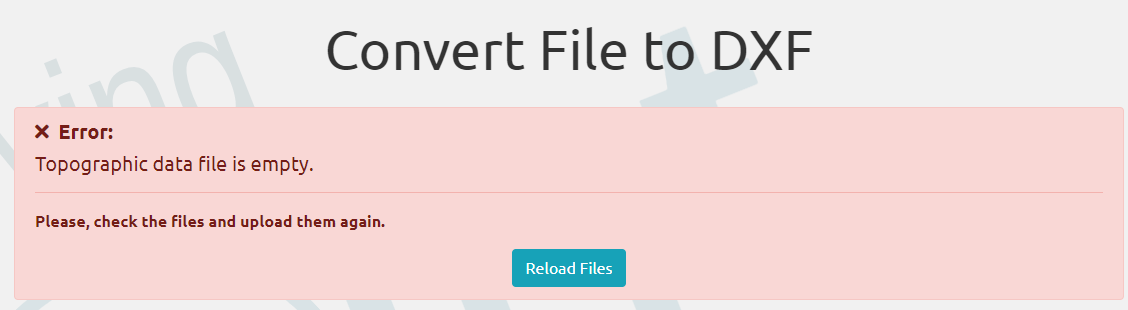
\includegraphics[width=0.7\textwidth]{M_07_E6}
	\caption{Error archivo topográfico vacío.}
	\label{fig:M_07_E6}
\end{figure}

\item El número de puntos para definir cuadrados con el código <<TC>> no es un numero par, por lo que no se puede garantizar la generación correcta de estos elementos. Se da la opción de volver a cargar el archivo, pulsando el botón \emph{Reload Files}.

\begin{figure}[H]
	\centering
	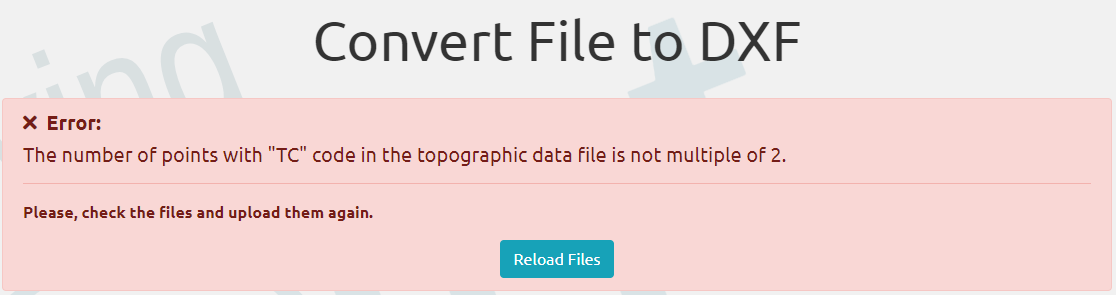
\includegraphics[width=0.7\textwidth]{M_07_E1}
	\caption{Error archivo topográfico, dibujo de cuadrados.}
	\label{fig:M_07_E1}
\end{figure}

\item El número de puntos para definir rectángulos con el código <<TR>> no es múltiplo de 3, por lo que no se puede garantizar la generación correcta de estos elementos. Se da la opción de volver a cargar el archivo, pulsando el botón \emph{Reload Files}.

\begin{figure}[H]
	\centering
	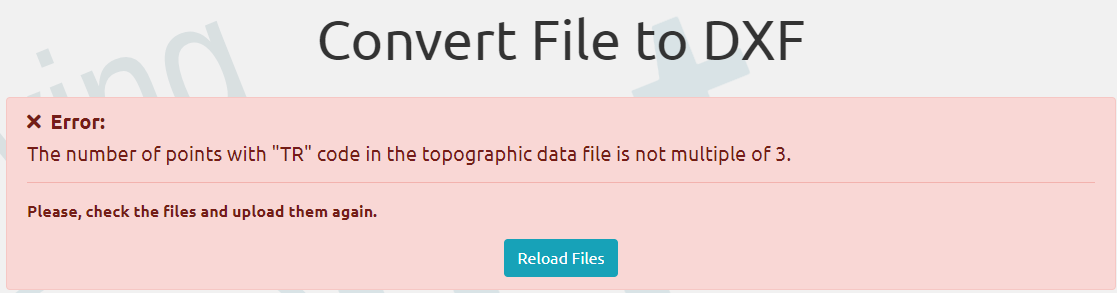
\includegraphics[width=0.7\textwidth]{M_07_E4}
	\caption{Error archivo topográfico, dibujo de rectángulos.}
	\label{fig:M_07_E4}
\end{figure}

\end{itemize}


\subsubsection{Carga de archivo de configuración de la conversión.}

El archivo de configuración de la conversión \textbf{no es obligatorio} para generar un archivo DXF a partir de un levantamiento topográfico. El archivo estará compuesto por una o varias líneas, cada línea equivale a una configuración para un código de campo. Cada línea o configuración estará formado por los siguientes campos, unos obligatorios y otro opcional, separados por comas:

\begin{itemize}
\item Código topográfico.
\item Capa de CAD.
\item Color.
\item Símbolo. Este campo es opcional
\end{itemize}

A continuación vemos un ejemplo de un archivo:

\begin{verbatim}
CA,Cañada,(255,0,0)
VA,Valla,(255,255,0)
ARB,Arbol,(0, 255, 127),Arbol
P,Hidrología,(0,127,255),Pozo
L,Hidrología,(0,127,255)
E,Edificio,(255, 0,255)
TO,Torreta,(0,0,0),Torreta_Media
EXD,Expropiación,(0,0,0)
EXI,Expropiación,(0,0,0)
CAD,Canal,(0,0,255)
CAI,Canal,(0,0,255)
LEM,Línea_Eléctrica_Media,(255,63,0),Torreta_Media
LEA,Línea_Eléctrica_Alta,(204,204,102),Torreta_Alta
SAN,Saneamiento,(255, 0, 255)
AC,Acera,(255,255,0)

\end{verbatim}



\textbf{\underline{Pasos para cargar un archivo de configuración de la conversión:} }

\begin{enumerate}

\item Debe haber un archivo topográfico seleccionado.
\item Elegir un archivo de configuración de la conversión.
\item Pulsar el botón \emph{Upload}

Si el archivo es correcto, la aplicación irá a la pantalla \emph{Convert File to DXF}.

\end{enumerate}

\textbf{\underline{Errores en la carga del archivo:} } 

La carga no será correcta si al pulsar el botón \emph{Upload}, se presentan los siguientes errores:

\begin{itemize}


\item El archivo no tiene el formato correcto. En el mensaje aparecen las líneas del archivo donde están los errores. Se da la opción de volver a cargar el archivo, pulsando el botón \emph{Reload Files}.

\begin{figure}[H]
	\centering
	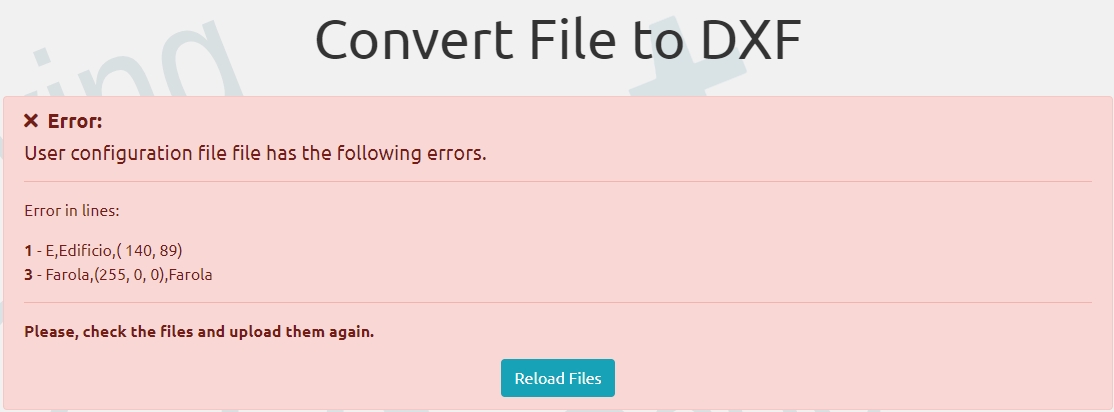
\includegraphics[width=0.7\textwidth]{M_07_E2}
	\caption{Error formato de archivo configuración de la conversión, \emph{parser}.}
	\label{fig:M_07_E2}
\end{figure}

\item El archivo está vacío. Se da la opción de volver a cargar el archivo, pulsando el botón \emph{Reload Files}.

\begin{figure}[H]
	\centering
	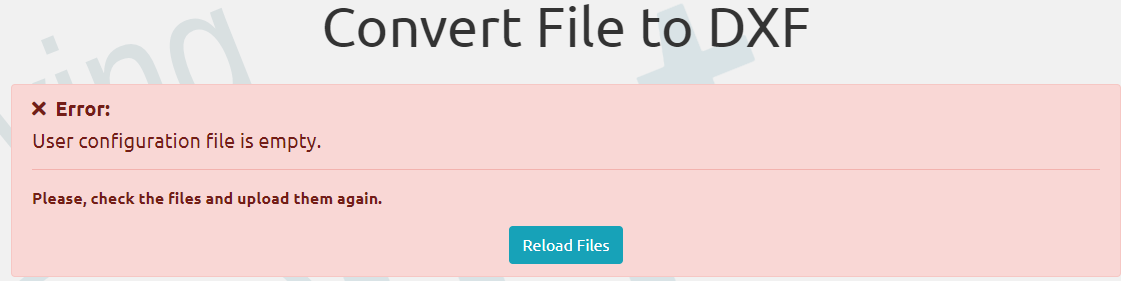
\includegraphics[width=0.7\textwidth]{M_07_E5}
	\caption{Error archivo configuración de la conversión vacío.}
	\label{fig:M_07_E5}
\end{figure}

\item Un mismo tipo de código topográfico, aparece repetido en diferentes líneas. Se da la opción de volver a cargar el archivo, pulsando el botón \emph{Reload Files}.

\begin{figure}[H]
	\centering
	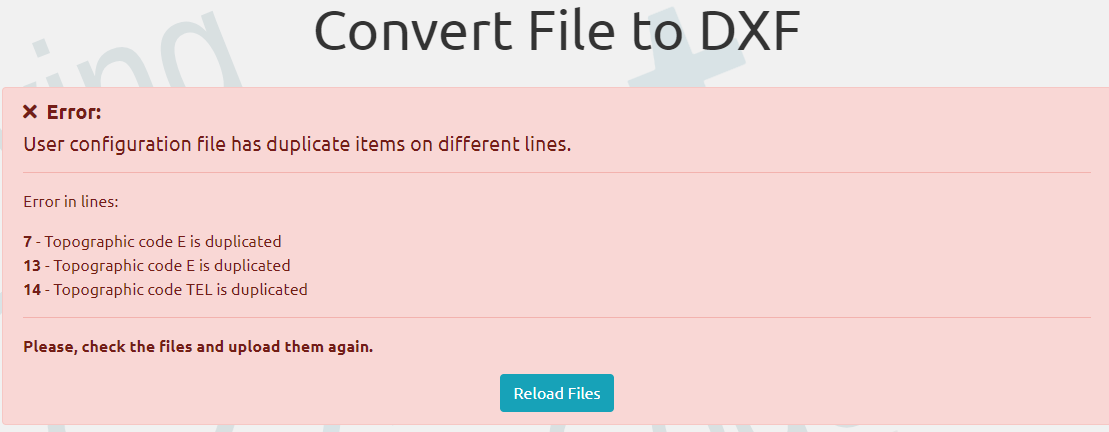
\includegraphics[width=0.7\textwidth]{M_07_E3}
	\caption{Error archivo configuración de la conversión, códigos repetidos.}
	\label{fig:M_07_E3}
\end{figure}

\item Los errores siguientes permiten al usuario corregir estos a través de la interfaz, sin necesidad de volver a cargar el archivo:

\begin{enumerate}
\item Una capa con el mismo nombre, tiene diferentes colores asignados. El mensaje de error muestra la capa que es errónea.

\item El archivo de configuración de la conversión contiene colores que no pertenecen a la paleta de CAD. El mensaje de error muestra la capa que es y el color asignado erróneo.

\end{enumerate}
\begin{figure}[H]
	\centering
	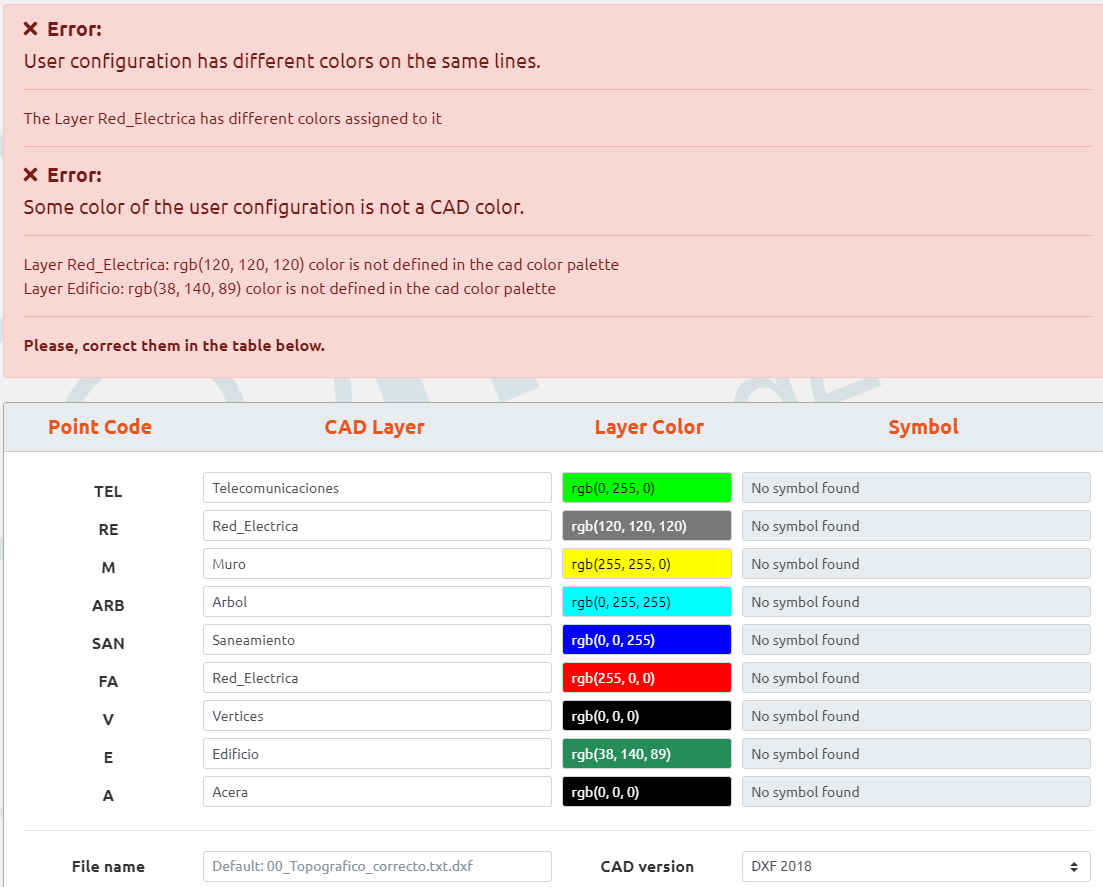
\includegraphics[width=0.7\textwidth]{M_08_E}
	\caption{Errores corregibles a través de la interfaz.}
	\label{fig:M_08_E}
\end{figure}

\end{itemize}

\subsubsection{Carga de archivo de símbolos.}

El archivo de símbolos \textbf{no es obligatorio} para generar un archivo DXF a partir de un levantamiento topográfico. El archivo estará compuesto por uno o varios bloques.

\begin{enumerate}

\item Debe haber un archivo topográfico seleccionado.
\item Elegir un archivo de símbolos.
\item Pulsar el botón \emph{Upload}

Si el archivo es correcto, la aplicación irá a la pantalla \emph{Convert File to DXF}.

\end{enumerate}

\textbf{\underline{Errores en la carga del archivo:} } 

La carga no será correcta si al pulsar el botón \emph{Upload}, se presentan los siguientes errores:

\begin{itemize}


\item El archivo está vacío. Puede ser un archivo con formato DXF correcto, pero \textbf{no contener ninguna entidad bloque}, por lo que la aplicación no podrá interpretar los símbolos. Se da la opción de volver a cargar el archivo, pulsando el botón \emph{Reload Files}.

\begin{figure}[H]
	\centering
	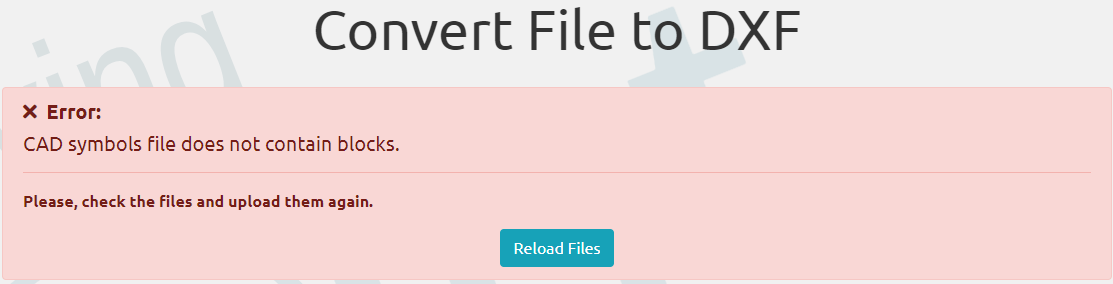
\includegraphics[width=0.7\textwidth]{M_07_E7}
	\caption{Error archivo de símbolos, no contiene bloques.}
	\label{fig:M_07_E7}
\end{figure}

\end{itemize}

\subsection{Conversión a DXF.}


\textbf{\underline{Pasos para realizar la conversión a un archivo DXF:} }

\begin{enumerate}


\item El usuario podrá introducir o modificar, los nombres de las capas, colores y símbolos (si se ha cargado un archivo con simbología), a través de la interfaz. 
\begin{figure}[H]
	\centering
	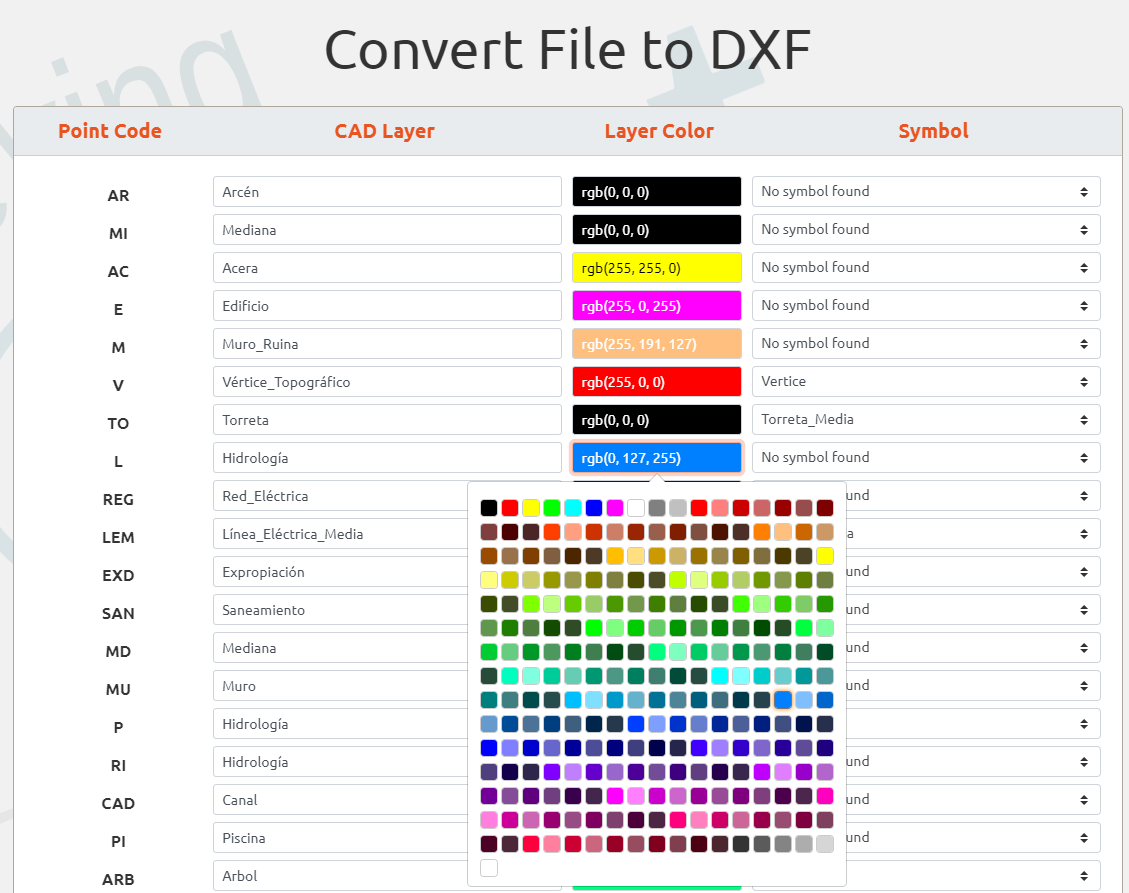
\includegraphics[width=0.7\textwidth]{M_08}
	\caption{Elección de colores.}
	\label{fig:M_08}
\end{figure}

\begin{figure}[H]
	\centering
	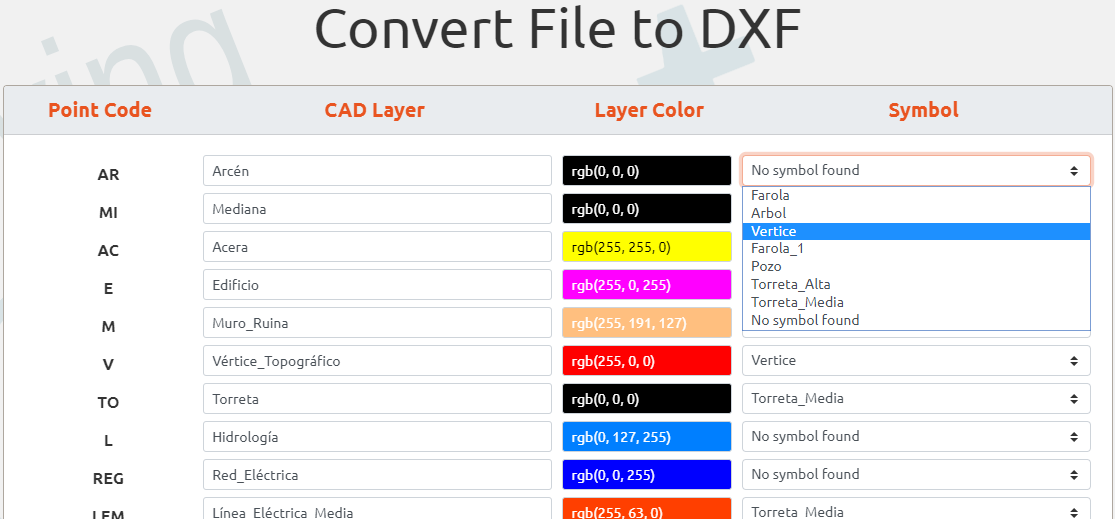
\includegraphics[width=0.7\textwidth]{M_09}
	\caption{Elección de símbolos.}
	\label{fig:M_09}
\end{figure}

\item El usuario podrá asignar un nombre al archivo DXF generado, introduciendo el nombre en la caja \emph{File name}. Si no le asigna un nombre, se le asignará por defecto el nombre del archivo topográfico cargado.


\item El usuario podrá elegir la versión de CAD que desea que tenga el DXF generado. Si no le asigna ninguna, se le asignará por defecto la versión CAD 2018 (AC1032).

\begin{figure}[H]
	\centering
	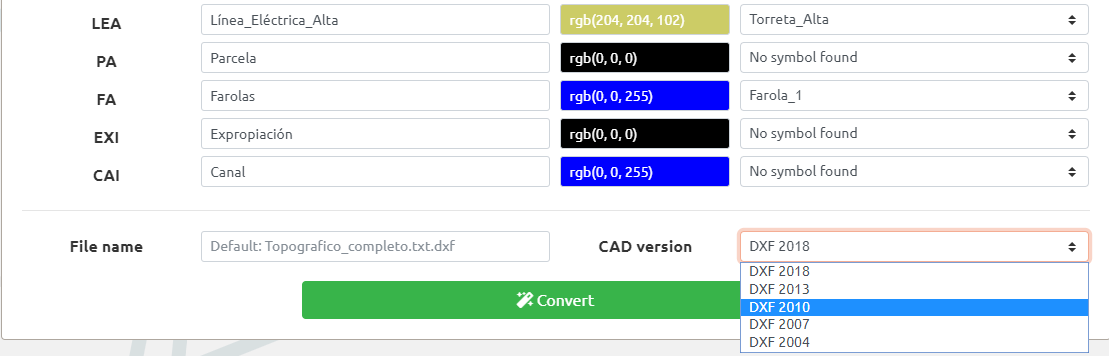
\includegraphics[width=0.7\textwidth]{M_10}
	\caption{Elección de versión de CAD.}
	\label{fig:M_10}
\end{figure}

\item Por último, el usuario pulsará el botón \textbf{Convert} y si todo es correcto, la aplicación irá a la pantalla \emph{Download File} y mostrará un mensaje informando que la conversión se ha realizado con éxito.

\begin{figure}[H]
	\centering
	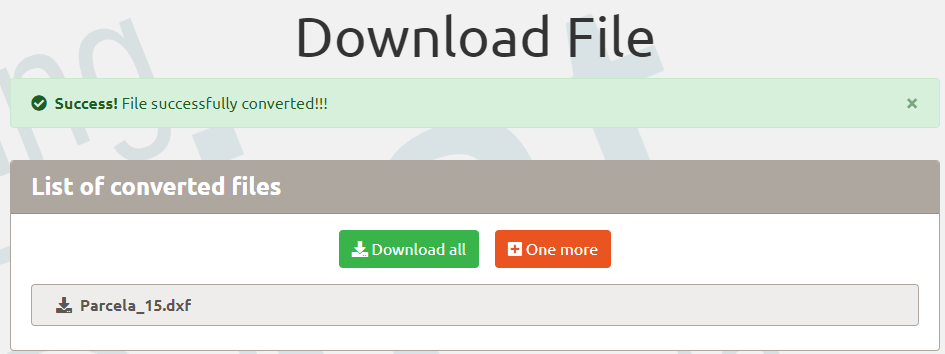
\includegraphics[width=0.7\textwidth]{M_11}
	\caption{Conversión con éxito.}
	\label{fig:M_11}
\end{figure}

\end{enumerate} 

\textbf{\underline{Errores en la conversión del archivo:} } 

La conversión no se podrá realizar si al pulsar el botón \emph{Convert}, se presentan los siguientes errores:

\begin{enumerate}
\item Una capa con el mismo nombre, tiene diferentes colores asignados. El mensaje de error muestra la capa que es errónea.

\item El archivo de configuración de la conversión contiene colores que no pertenecen a la paleta de CAD. El mensaje de error muestra la capa que es y el color asignado erróneo.

\end{enumerate}
\begin{figure}[H]
	\centering
	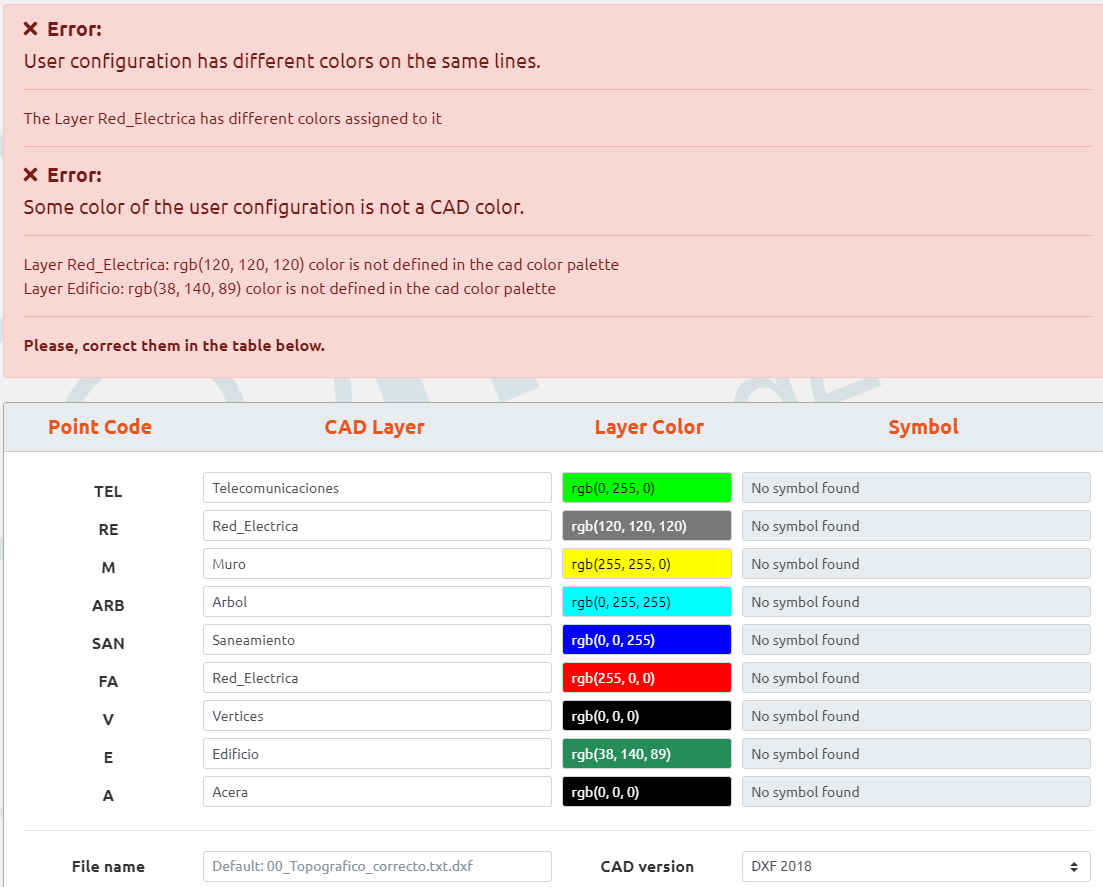
\includegraphics[width=0.7\textwidth]{M_08_E}
	\caption{Errores corregibles a través de la interfaz.}
	\label{fig:M_08_E}
\end{figure}

\subsection{Descarga de archivos.}


\textbf{\underline{Pasos para realizar la descarga de archivos:} }

\begin{enumerate}

\item Si el usuario desea descargar un archivo de forma individual, pulsará sobre el nombre del archivo que aparece en la lista de archivos convertidos. A continuación el archivo se descargará a su equipo.

\item Si el usuario desea descargar varios archivos a la vez, en formato comprimido, pulsará sobre el botón \emph{Download all}. A continuación el archivo comprimido se descargará a su equipo.

\begin{figure}[H]
	\centering
	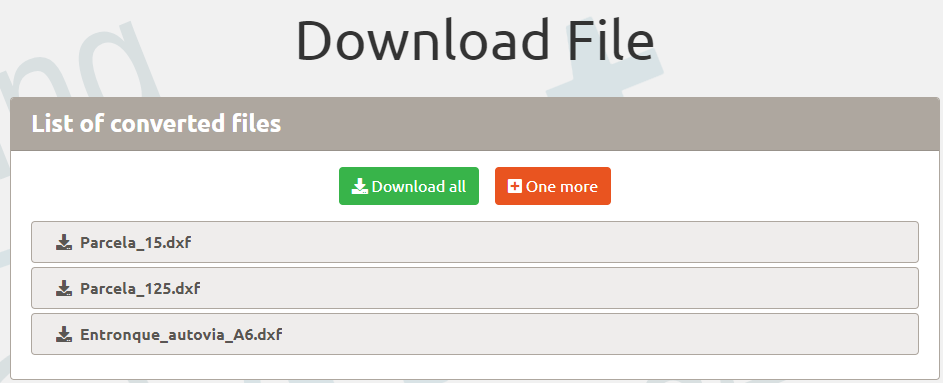
\includegraphics[width=0.7\textwidth]{M_12}
	\caption{Descarga de archivos.}
	\label{fig:M_12}
\end{figure}

\end{enumerate} 


\newpage
\textbf{\underline{Otras opciones:} }

\begin{itemize}

\item El usuario puede seguir convirtiendo archivos pulsando el botón \emph{One more}.

\end{itemize}

\subsection{\emph{Logout}.}


\textbf{\underline{Cerrar la sesión de usuario:} }

\begin{itemize}

\item El usuario puede cerrar la sesión pulsando el botón \emph{Sign out}, situado en el menú desplegable de la barra de navegación superior. La sesión de usuario se cerrará y la aplicación irá a la pantalla de bienvenida.

\begin{figure}[H]
	\centering
	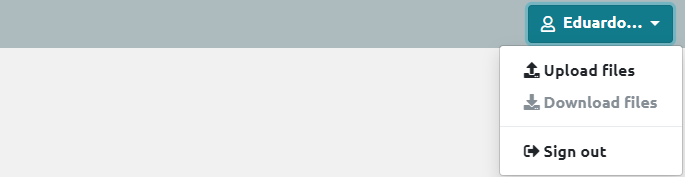
\includegraphics[width=0.7\textwidth]{M_05_A}
	\caption{\emph{Logout}}
	\label{fig:M_05_A}
\end{figure}

\item Una vez \emph{logeado} el usuario, puede cerrar su sesión desde cualquier pantalla de la aplicación.

\item La sesión de usuario se cerrará tras 5 minutos de inactividad en la aplicación y volverá a la pantalla de \emph{login}
\begin{figure}[H]
	\centering
	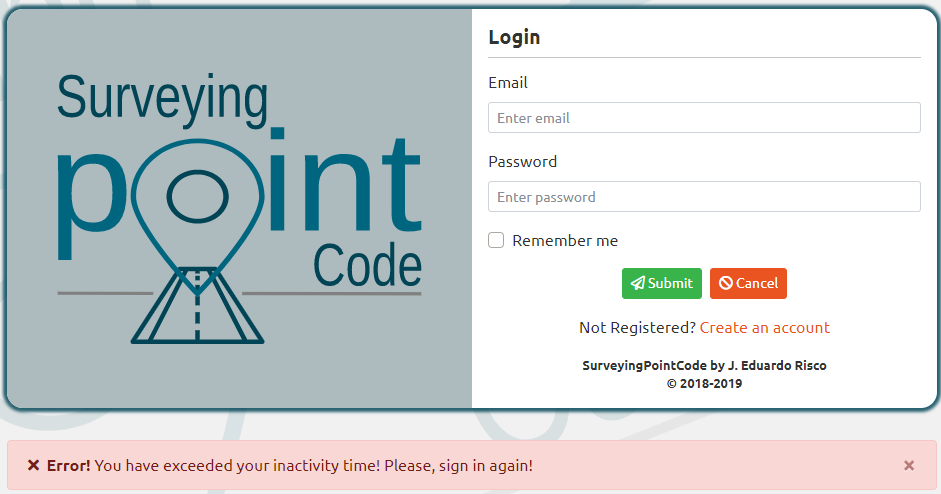
\includegraphics[width=0.7\textwidth]{M_13}
	\caption{\emph{Cierre de sesión por inactividad}}
	\label{fig:M_13}
\end{figure}

\end{itemize}
\newpage
\section{Preguntas Frecuentes}

\begin{itemize}
\item \textbf{\textbf{¿Es necesario registrarse en la aplicación?}} Sí, es necesario registrarse para poder usar la aplicación.

\item \textbf{\textbf{¿Se pueden convertir archivos sin códigos?}} No, el archivo debe contener códigos. Todos los puntos deben tener asociado un código. La aplicación mostrará un error.

\item \textbf{\textbf{¿Es necesario cargar un archivo de configuración de la conversión para generar un archivo DXF?}} No, no es necesario. Se puede configurar la conversión a través de la interfaz.

\item \textbf{\textbf{¿Es necesario cargar un archivo de símbolos para generar un archivo DXF?}} No, no es necesario. El archivo generado no contendrá ningún símbolo.

\item \textbf{\textbf{¿Es necesario configurar una conversión, asociando capas, colores y símbolos, para generar un archivo DXF?}} No, no es necesario. Si no se definen asociaciones, el archivo generado guardará todos los elementos por defecto en la capa \textbf{Layer 0}, con color \textbf{RGB(0,0,0)} y sin ningún símbolo asociado.

\item \textbf{\textbf{¿Es necesario dar un nombre al archivo DXF a generar?}} No, no es necesario. Si no se le asigna nombre, el archivo generado se guardará por defecto con el nombre del archivo topográfico.

\item \textbf{\textbf{¿Es necesario seleccionar una versión de CAD para generar el archivo DXF?}} No, no es necesario. Si no se selecciona una versión, el archivo generado se creará por defecto con la versión \textbf{CAD 2018}.

\item \textbf{\textbf{¿Es posible asociar diferentes códigos topográficos a una misma capa de CAD?}} Sí, por ejemplo los códigos: P, CA y RI, que pueden significar: pozo, canal y río, se pueden asociar a la única capa Hidrología.

\item \textbf{\textbf{¿Es posible asociar el mismo código topográfico a diferentes capas de CAD?}} No, no es posible. La aplicación mostrará un error.

\item \textbf{\textbf{¿Es posible asociar distintos colores a al misma capa de CAD?}} No, no es posible. La aplicación mostrará un error.

\item \textbf{\textbf{¿Es posible asociar cualquier color a una capa de CAD?}} No, no es posible. Solo los colores de la paleta CAD. La aplicación mostrará un error. 

Los colores disponibles se pueden consultar en: \url{http://gohtx.com/acadcolors.php}

\item \textbf{\textbf{Si se nos olvida cerrar la sesión. ¿Nuestra sesión permanecerá permanentemente abierta?}} No, la sesión se cerrará por seguridad, al cabo de 5 minutos de inactividad.
\end{itemize}